\section{A tecnologia blockchain}
\subsection{Estrutura e funcionamento da blockchain}

\begin{frame}{Blockchain}
    \begin{block}{}
    \textbf{Blockchain} é o nome dado à tecnologia subjacente utilizada em diversas plataformas
    de gerenciamento descentralizado de posse de bens digitais baseada em \textbf{livro-razão distribuído}
    (do inglês, \textbf{\textit{Distributed Ledger Technology}} (DLT) )
    \end{block}
    Principais características:
    \begin{itemize}
        \item Armazenamento descentralizado e distribuído;
        \item Imutabilidade;
        \item Transparência;
        \item Dispensa da necessidade de confiança em uma terceira parte.
    \end{itemize}
\end{frame}

\begin{frame}{Blockchain Bitcoin}
    \begin{itemize}
        \item Primeiro caso de êxito: \textbf{Bitcoin};%\footnotemark[1];
            \item Criada em 2008 por Satoshi Nakamoto;
            \item Criptomoeda gerada e gerenciada de forma distribuída;
            \item Não possui entidades centralizadoras;
            \item Formada por uma rede de nós conectados auto-gerenciáveis;
            \item Nós trabalham para manter a integridade do sistema;
    \end{itemize}  
\end{frame}

\begin{frame}{Blockchain - Transações e blocos}
    \begin{itemize}
        \item Sempre que a posse de uma unidade ou fração de Bitcoin é transferida, uma \textbf{transação} é gerada;
        \item Quando uma nova transação ocorre, suas informações são transmitidas pela rede, tais como:
        \begin{itemize}
            \item Contas envolvidas;
            \item Quantia transferida;
            \item Assinatura digital;
            \item Horário da transação.
        \end{itemize}
        \item Os nós da rede, conhecidos como \textbf{mineradores}, coletam as transações e as armazenam em \textbf{blocos};
        \item Transações de um bloco são organizadas eu uma \textbf{árvore de Merkle}:
            \begin{itemize}
                \item Nós folhas: transações;
                \item Demais nós: Referências de \textit{hash}.
            \end{itemize}
    \end{itemize}
\end{frame}

\begin{frame}{Blockchain - Estrutura}
    \begin{figure}[!htb]
     \centering
     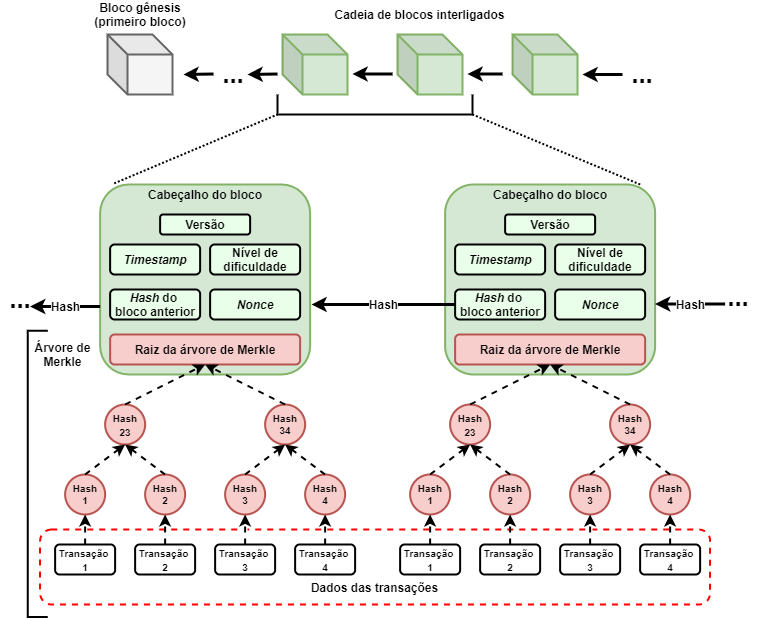
\includegraphics[scale=0.3]{figuras/blockchain/block_estrutura_cabeçalho.png}
    \end{figure}    
\end{frame}

\begin{frame}{Blockchain - Validação dos blocos}
    \begin{block}{Algoritmo de consenso}
    \begin{itemize}
        \item Regras a serem seguidas pelos nós para criação e validação dos blocos;
        \item Recompensa para os nós honestos;
        \item Garante que todos os nós da rede concordem com o histórico de transações que compõem os blocos da blockchain.
    \end{itemize}
    \end{block}    
\end{frame}

\begin{frame}{Blockchain - Algoritmos de consenso}
    \begin{exampleblock}{\textit{Proof-of-Work} (PoW)}
    \begin{itemize}
        \item Utilizado nas blockchains Bitcoin e Ethereum;
        \item Consiste na competição entre os mineradores para resolução do \textit{nonce} do bloco;
        \item O vencedor transmite o bloco pela rede para validação;
        \item Quanto maior o poder computacional do minerador, maior a chance de vencer;
        \item Resulta em um alto esforço computacional e gasto energético;
        \item O vencedor receber um valor da criptomoeda como recompensa (e.g., Bitcoin);
        \item \textbf{Desvantagem}: Esforço computacional elevado.
    \end{itemize}
    \end{exampleblock}
\end{frame}

% no final da explicação de blockchain, fazer um slide falando pq é difícil fraudar um bloco

\subsection{Blockchain Ethereum}

\begin{frame}{Ethereum}
    \begin{block}{}
    \begin{itemize}
        \item Apesar da blockchain ter sido criada para uma aplicação financeira (i.e., a Bitcoin), seus conceitos e protocolos podem ser estendidos para diversas áreas;
        \item É apenas um fim para um meio;
        \item Aplicações: Cuidados médicos, inteligência artificial, internet das coisas, governança descentralizada, entre outras.
    \end{itemize}
    \end{block}
    \begin{block}{}
    \begin{itemize}
        \item Em 2014 foi criada a blockchain \textbf{Ethereum};
        \item Introdução dos contratos inteligentes;
        \item Pioneira na expansão das aplicações da blockchain.
    \end{itemize}
    \end{block}
\end{frame}

\begin{frame}{Ethereum}
    \begin{itemize}
        \item Permite a geração, transferência e gerenciamento de sua criptomoeda, o \textbf{Ether};
        \item Seu funcionamento é baseado na implantação dos \textbf{contratos inteligentes} (CI):
        \begin{itemize}
            \item Programas de computador;
            \item Executam automatica e obrigatoriamente aquilo que foi programado;
            \item Estabelecem um acordo entre os envolvidos;
            \item Geração de transações.
        \end{itemize}
	    \item Opera de forma semelhante à Bitcoin na garantia da \textbf{imutabilidade}.
    \end{itemize}
\end{frame} 

%\begin{frame}{Ethereum}
%    \begin{itemize}
%        \item Aplicações Descentralizadas (do inglês, \textit{Descentralized Applications} (DApps)):
%        \begin{itemize}
%            \item Mais de 3 mil utilizam a Ethereum~\footnote{\url{<https://www.stateofthedapps.com/>}}.
%        \end{itemize}
%    \end{itemize}
%\end{frame}

\begin{frame}{Ethereum - Propriedades}
    As aplicações que executam sobre a Ethereum dispõem de uma série de propriedades:
    \begin{itemize}
        \item Descentralização;
        \item Imutabilidade;
        \item Persistência de dados;
        \item Execução autônoma;
        \item Acurácia.
    \end{itemize}
\end{frame}

\begin{frame}{Ethereum - Aplicações}
    \begin{itemize}
        \item Sistema de \textbf{tokens}:
        \begin{itemize}
            \item Tokenização;
            \item Padrão ERC-20.
        \end{itemize}
        \item Organização Autônoma Descentralizada:
        \begin{itemize}
            \item Regras operacionais e de gerenciamento são programadas em um CI;
            \item Abolição de modelos baseados em hierarquia;
            \item Redução de custos;
            \item Primeira OAD: \textit{The DAO}.
        \end{itemize}
        \item Cuidados médicos e serviços de saúde:
        \begin{itemize}
            \item Integração de dados de prontuários.
        \end{itemize}
    \end{itemize}
\end{frame}

%\begin{frame}{Ethereum - Arquitetura em camadas}
%    \begin{figure}[!htb]
%     \centering
%     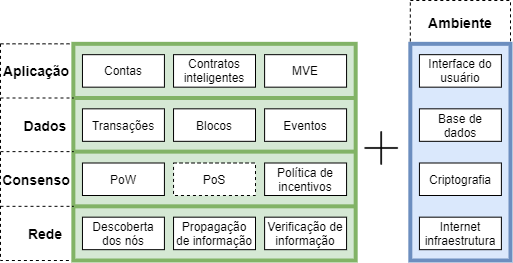
\includegraphics[scale=0.5]{figuras/blockchain/ethereum_arquitetura.png}
%    \end{figure}    
%\end{frame}